\documentclass{article}
\usepackage{listings}
\usepackage{graphicx}
\author{Yuxiang Chen 5110309783}
\title{Report of Lab9}
\begin{document}
\maketitle
\tableofcontents
\section{The Purpose of This Experiment}
In this experiment, our main purpose is to use a hash table to eliminate the time when we try to match a certain picture. Usually, we use the method referred in the pdf files of establishing a twelve-dimension vector for each picture we're to search, and then compare them with each other, getting the one that is the most similar. However, this may lead to a waste of time when we just compare these pictures one by one. So in order to save time, we may just get a part of their characters and set up a hash table using which we can promptly find the certain group that has the same feature with the target. Thus we can spare quite a lot time. So in this experiment. we need to use the LSH method to accomplish our goal to save time and make it easy when matching pictures.
\section{The Main Part of the Experiment}
Since we have to compare the effect of those two method, I write two programs. One for the normal NN or KNN method, and the other for LSH. And at last I print out the matched result and the time used in the searching program.
\subsection{The method of KNN}
This method is the so-called 'violent' method, since we just compare the twelve-dimension vector of them and if they're the same, we can judge that the two pictures are similar. Although this is a correct method, it really wastes time since it will also compare those graphs which is definitely has no similarity with the target.\\
In this part, I calculate the percentage of green, red and blue in the four parts of the picture, and they consist the twelve-dimension vector we need. Then I change it into the '0 1 2' form we need. And following are my codes:
\begin{lstlisting}[language=python,numbers=left,frame=leftline]
import sys
import string
import time
from opencv.cv import *
from opencv.highgui import *

def get_data(filename):
    twelve=list()
    p=list()
    image = cvLoadImage (filename,1)
    width=image.width
    height=image.height
    semi_w=width/2
    semi_h=height/2
    red=0
    green=0
    blue=0
    for i in range(0,semi_w):
        for j in range(0,semi_h):
            red+=image[j,i][2]
            blue+=image[j,i][0]
            green+=image[j,i][1]
    total=red+green+blue
    p.append(float(blue)/total)
    p.append(float(green)/total)
    p.append(float(red)/total)
    red=0
    green=0
    blue=0
    for i in range(0,semi_w):
        for j in range(semi_h,height):
            red+=image[j,i][2]
            blue+=image[j,i][0]
            green+=image[j,i][1]
    total=red+green+blue
    p.append(float(blue)/total)
    p.append(float(green)/total)
    p.append(float(red)/total)
    red=0
    green=0
    blue=0
    for i in range(semi_w,width):
        for j in range(0,semi_h):
            red+=image[j,i][2]
            blue+=image[j,i][0]
            green+=image[j,i][1]
    total=red+green+blue
    p.append(float(blue)/total)
    p.append(float(green)/total)
    p.append(float(red)/total)
    red=0
    green=0
    blue=0
    for i in range(semi_w,width):
        for j in range(semi_h,height):
            red+=image[j,i][2]
            blue+=image[j,i][0]
            green+=image[j,i][1]
    total=red+green+blue
    p.append(float(blue)/total)
    p.append(float(green)/total)
    p.append(float(red)/total)
    for k in range(0,12):
        if p[k]>=0 and p[k]<0.3:
            twelve.append(0)
        if p[k]>=0.3 and p[k]<0.6:
            twelve.append(1)
        if p[k]>=0.6:
            twelve.append(2)
    return twelve

def get_all_twelve():
    total_vector=list()
    for t in range(1,41):
        filename=str(t)+".jpg"
        twelve=get_data(filename)
        total_vector.append(twelve)
    return total_vector

def get_all_target():
    new_twelve=get_data("target.jpg")
    return new_twelve

total_vector=get_all_twelve()
new_twelve=get_all_target()
start=time.clock()
for i in range(0,40):
    if total_vector[i]==new_twelve:
        print "The picture is "+str(i+1)+".jpg"
end=time.clock()
delta=end-start
print "time:",delta
\end{lstlisting}
And after this program, I get the result like this picture. But we get two result, the program thinks that both 12.jpg and 38.jpg is similar to the target. And if we see it carefully, 12.jpg, although not the exact graph, really resembles our target in some way. Whatever, as the method itself is to find the similar result, not the exact one, so we can think it attain the expectation we want.
\begin{figure}[htbp]
\centering
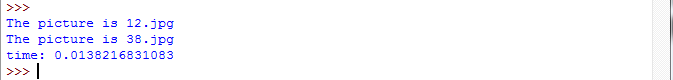
\includegraphics[width=10cm]{knn1.png}
\caption{The result of KNN} 
\end{figure}
\subsection{The method of LSH}
In this part, we have to make an hash table which contains some feature of the pictures, say, maybe some digits of its vector. And then if we use the hash function we establish and get a key, then search the key to get a certain bin in the data base. And in this way, we find the bin which the graph most similar to our target in. So we can just use the KNN method to search this bin, but with less samples to traverse. Thus we can save much time.\\
And in this section, I first make a hash table of the data base given, then just find which bin the target is in. And then the program is just the same as the first one, finding the result by comparing the twelve-dimension vector. I set the projection to be {1,3,7,8} by default, you can modify it directly in the program if you want, and my program will get the new hamming code automatically. Here are my codes:
\begin{lstlisting}[language=python,numbers=left,frame=leftline]
import sys
import string
import time
from opencv.cv import *
from opencv.highgui import *
#���������C=2��d=12,d'=24
I=[1,3,7,8]#����ֻҪ�޸�I�����ݣ�����ij�����Զ������Ӧ��hamming��
c=2
projection=dict()
for i in range(1,13):
    for num in I:
        if (i-1)*c+1<=num and num<=i*c:
            if projection.has_key(str(i)):
                projection[str(i)].append(num)
            else:
                projection[str(i)]=[num]
hashkeys=projection.keys()

def get_data(filename):
    twelve=list()
    p=list()
    image = cvLoadImage (filename,1)
    width=image.width
    height=image.height
    semi_w=width/2
    semi_h=height/2
    red=0
    green=0
    blue=0
    for i in range(0,semi_w):
        for j in range(0,semi_h):
            red+=image[j,i][2]
            blue+=image[j,i][0]
            green+=image[j,i][1]
    total=red+green+blue
    p.append(float(blue)/total)
    p.append(float(green)/total)
    p.append(float(red)/total)
    red=0
    green=0
    blue=0
    for i in range(0,semi_w):
        for j in range(semi_h,height):
            red+=image[j,i][2]
            blue+=image[j,i][0]
            green+=image[j,i][1]
    total=red+green+blue
    p.append(float(blue)/total)
    p.append(float(green)/total)
    p.append(float(red)/total)
    red=0
    green=0
    blue=0
    for i in range(semi_w,width):
        for j in range(0,semi_h):
            red+=image[j,i][2]
            blue+=image[j,i][0]
            green+=image[j,i][1]
    total=red+green+blue
    p.append(float(blue)/total)
    p.append(float(green)/total)
    p.append(float(red)/total)
    red=0
    green=0
    blue=0
    for i in range(semi_w,width):
        for j in range(semi_h,height):
            red+=image[j,i][2]
            blue+=image[j,i][0]
            green+=image[j,i][1]
    total=red+green+blue
    p.append(float(blue)/total)
    p.append(float(green)/total)
    p.append(float(red)/total)
    for k in range(0,12):
        if p[k]>=0 and p[k]<0.3:
            twelve.append(0)
        if p[k]>=0.3 and p[k]<0.6:
            twelve.append(1)
        if p[k]>=0.6:
            twelve.append(2)
    return twelve

def get_all_twelve():
    total_vector=list()
    for t in range(1,41):
        filename=str(t)+".jpg"
        twelve=get_data(filename)
        total_vector.append(twelve)
    return total_vector

def get_all_target():
    new_twelve=get_data("target.jpg")
    return new_twelve

def get_hash_key(vector,hashkeys):
    key=list()
    for j in range(0,len(hashkeys)):
        x=vector[int(hashkeys[j])-1]
        for num in projection[hashkeys[j]]:
            if num-c*(int(hashkeys[j])-1)<=x:
                key.append(1)
            else:
                key.append(0)
    return key

def get_hash(total_vector,projection):
    hash_dict={}
    for i in range(0,40):
        key=get_hash_key(total_vector[i],hashkeys)
        if hash_dict.has_key(str(key)):
            hash_dict[str(key)].append(i)
        else:
            hash_dict[str(key)]=[i]
    return hash_dict

def get_target_hash(newtwelve):
    new_key=get_hash_key(newtwelve,hashkeys)
    return new_key

if __name__ == '__main__':
    total_vector=get_all_twelve()
    newtwelve=get_all_target()
    hash_dict=get_hash(total_vector,projection)
    newkey=get_target_hash(newtwelve)
    start=time.clock()
    result_set=hash_dict[str(newkey)]
    for num in result_set:
        if newtwelve==total_vector[num]:
            print "The picture is "+str(num+1)+".jpg"
    end=time.clock()
    delta=end-start
    print "time:",delta
\end{lstlisting}
And in this part I get the same result as the KNN method -- two result. But there's a significant time-drop by using this method. So we can just believe this method can save us lots of time when the data base is big enough. And then I change the projection to be {2,3,7,10} and still get the same result. Here are the screenshots.
\begin{figure}[htbp]
\centering
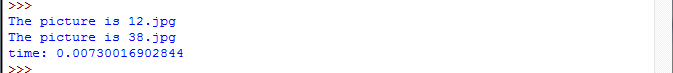
\includegraphics[width=10cm]{lsh1.png}
\caption{The result of 1,3,7,8}
\end{figure}
\begin{figure}[htbp]
\centering
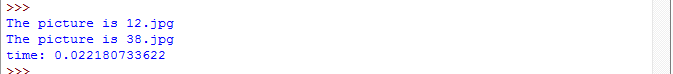
\includegraphics[width=10cm]{lsh23710.png}
\caption{The result of 2,3,7,10}
\end{figure}
\section{The Problems I Met and My Thoughts}
As the last program in this semester, I feel happy to accomplished it in time all by myself, as all of the former codes. So after finishing this program, what I realise first is the importance of make a structure like a directory when searching files. Since in this way, we can largely eliminate the time used in some unrelated objects. And since the experiment isn't very difficult, so I didn't meet much trouble at first. After understanding what the question means, I directly write it. And at last, I feel very thankful for TA's generous help when I emailed him for some questions. Of course, although the course is over, I will keep on learning about image processing, since I think there's a lot fun in it. Thank you.
\end{document} 